\documentclass{ximera}

\title{Practice for Eigenvalue Method with Repeated Roots}

%\auor{Matthew Charnley and Jason Nowell}
\usepackage[margin=1.5cm]{geometry}
\usepackage{indentfirst}
\usepackage{sagetex}
\usepackage{lipsum}
\usepackage{amsmath}
\usepackage{mathrsfs}


%%% Random packages added without verifying what they are really doing - just to get initial compile to work.
\usepackage{tcolorbox}
\usepackage{hypcap}
\usepackage{booktabs}%% To get \toprule,\midrule,\bottomrule etc.
\usepackage{nicefrac}
\usepackage{caption}
\usepackage{units}

% This is my modified wrapfig that doesn't use intextsep
\usepackage{mywrapfig}
\usepackage{import}



%%% End to random added packages.


\graphicspath{
    {./figures/}
    {./../figures/}
    {./../../figures/}
}
\renewcommand{\log}{\ln}%%%%
\DeclareMathOperator{\arcsec}{arcsec}
%% New commands


%%%%%%%%%%%%%%%%%%%%
% New Conditionals %
%%%%%%%%%%%%%%%%%%%%


% referencing
\makeatletter
    \DeclareRobustCommand{\myvref}[2]{%
      \leavevmode%
      \begingroup
        \let\T@pageref\@pagerefstar
        \hyperref[{#2}]{%
	  #1~\ref*{#2}%
        }%
        \vpageref[\unskip]{#2}%
      \endgroup
    }%

    \DeclareRobustCommand{\myref}[2]{%
      \leavevmode%
      \begingroup
        \let\T@pageref\@pagerefstar
        \hyperref[{#2}]{%
	  #1~\ref*{#2}%
        }%
      \endgroup
    }%
\makeatother

\newcommand{\figurevref}[1]{\myvref{Figure}{#1}}
\newcommand{\figureref}[1]{\myref{Figure}{#1}}
\newcommand{\tablevref}[1]{\myvref{Table}{#1}}
\newcommand{\tableref}[1]{\myref{Table}{#1}}
\newcommand{\chapterref}[1]{\myref{chapter}{#1}}
\newcommand{\Chapterref}[1]{\myref{Chapter}{#1}}
\newcommand{\appendixref}[1]{\myref{appendix}{#1}}
\newcommand{\Appendixref}[1]{\myref{Appendix}{#1}}
\newcommand{\sectionref}[1]{\myref{\S}{#1}}
\newcommand{\subsectionref}[1]{\myref{subsection}{#1}}
\newcommand{\subsectionvref}[1]{\myvref{subsection}{#1}}
\newcommand{\exercisevref}[1]{\myvref{Exercise}{#1}}
\newcommand{\exerciseref}[1]{\myref{Exercise}{#1}}
\newcommand{\examplevref}[1]{\myvref{Example}{#1}}
\newcommand{\exampleref}[1]{\myref{Example}{#1}}
\newcommand{\thmvref}[1]{\myvref{Theorem}{#1}}
\newcommand{\thmref}[1]{\myref{Theorem}{#1}}


\renewcommand{\exampleref}[1]{ {\color{red} \bfseries Normally a reference to a previous example goes here.}}
\renewcommand{\figurevref}[1]{ {\color{red} \bfseries Normally a reference to a previous figure goes here.}}
\renewcommand{\tablevref}[1]{ {\color{red} \bfseries Normally a reference to a previous table goes here.}}
\renewcommand{\Appendixref}[1]{ {\color{red} \bfseries Normally a reference to an Appendix goes here.}}
\renewcommand{\exercisevref}[1]{ {\color{red} \bfseries Normally a reference to a previous exercise goes here.}}



\newcommand{\R}{\mathbb{R}}

%% Example Solution Env.
\def\beginSolclaim{\par\addvspace{\medskipamount}\noindent\hbox{\bf Solution:}\hspace{0.5em}\ignorespaces}
\def\endSolclaim{\par\addvspace{-1em}\hfill\rule{1em}{0.4pt}\hspace{-0.4pt}\rule{0.4pt}{1em}\par\addvspace{\medskipamount}}
\newenvironment{exampleSol}[1][]{\beginSolclaim}{\endSolclaim}

%% General figure formating from original book.
\newcommand{\mybeginframe}{%
\begin{tcolorbox}[colback=white,colframe=lightgray,left=5pt,right=5pt]%
}
\newcommand{\myendframe}{%
\end{tcolorbox}%
}

%%% Eventually return and fix this to make matlab code work correctly.
%% Define the matlab environment as another code environment
%\newenvironment{matlab}
%{% Begin Environment Code
%{ \centering \bfseries Matlab Code }
%\begin{code}
%}% End of Begin Environment Code
%{% Start of End Environment Code
%\end{code}
%}% End of End Environment Code


% this one should have a caption, first argument is the size
\newenvironment{mywrapfig}[2][]{
 \wrapfigure[#1]{r}{#2}
 \mybeginframe
 \centering
}{%
 \myendframe
 \endwrapfigure
}

% this one has no caption, first argument is size,
% the second argument is a larger size used for HTML (ignored by latex)
\newenvironment{mywrapfigsimp}[3][]{%
 \wrapfigure[#1]{r}{#2}%
 \centering%
}{%
 \endwrapfigure%
}
\newenvironment{myfig}
    {%
    \begin{figure}[h!t]
        \mybeginframe%
        \centering%
    }
    {%
        \myendframe
    \end{figure}%
    }


% graphics include
\newcommand{\diffyincludegraphics}[3]{\includegraphics[#1]{#3}}
\newcommand{\myincludegraphics}[3]{\includegraphics[#1]{#3}}
\newcommand{\inputpdft}[1]{\subimport*{../figures/}{#1.pdf_t}}


%% Not sure what these even do? They don't seem to actually work... fun!
%\newcommand{\mybxbg}[1]{\tcboxmath[colback=white,colframe=black,boxrule=0.5pt,top=1.5pt,bottom=1.5pt]{#1}}
%\newcommand{\mybxsm}[1]{\tcboxmath[colback=white,colframe=black,boxrule=0.5pt,left=0pt,right=0pt,top=0pt,bottom=0pt]{#1}}
\newcommand{\mybxsm}[1]{#1}
\newcommand{\mybxbg}[1]{#1}

%%% Something about tasks for practice/hw?
\usepackage{tasks}
\usepackage{footnote}
\makesavenoteenv{tasks}


%% For pdf only?
\newcommand{\diffypdfversion}[1]{#1}


%% Kill ``cite'' and go back later to fix it.
\renewcommand{\cite}[1]{}


%% Currently we can't really use index or its derivatives. So we are gonna kill them off.
\renewcommand{\index}[1]{}
\newcommand{\myindex}[1]{#1}







\begin{document}
\begin{abstract}
Why?
\end{abstract}
\maketitle



%Repeated eigenvalue, do not ask to solve a diffy q quite yet
\begin{exercise}
    Compute eigenvalues and eigenvectors of
    $\left[ 
        \begin{smallmatrix}
            -2 & -1 & -1 \\
            3 & 2 & 1 \\
            -3 & -1 & 0 \\
        \end{smallmatrix} 
    \right]$.\\
    $\lambda_1 = \answer{-2}$, $\vec{v}_1 = \left[\begin{smallmatrix} \answer{-1} \\ \answer{1} \\ -1 \end{smallmatrix}\right]$. $\lambda_2 = \answer{1}$, two-dimensional space of eigenvectors, options: $\left\{ \left[\begin{smallmatrix} \answer{-1} \\ 0 \\ \answer{3} \end{smallmatrix}\right],\ \left[\begin{smallmatrix} \answer{-1} \\ \answer{3} \\ 0 \end{smallmatrix}\right]\right\}$
\end{exercise}
%\comboSol
%{%
%$\lambda_1 = -2$, $\vec{v}_1 = \left[\begin{smallmatrix} -1 \\ 1 \\ -1 \end{smallmatrix}\right]$. $\lambda_2 = 1$, two-dimensional space of eigenvectors, options: $\left\{ \left[\begin{smallmatrix} -1 \\ 0 \\ 3 \end{smallmatrix}\right],\ \left[\begin{smallmatrix} -1 \\ 3 \\ 0 \end{smallmatrix}\right]\right\}$
%}

\begin{exercise}
    Let
    $A = \left[ 
        \begin{smallmatrix} 
            5 & -3 \\ 
            3 & -1 
        \end{smallmatrix} 
    \right]$.
    Find the general solution of ${\vec{x}}' = A \vec{x}$ and sketch the corresponding phase portrait.\\
    $\vec{x}(t) = C_1 \left[\begin{smallmatrix}  \answer{1} \\ \answer{1} \end{smallmatrix}\right]e^{2t} + C_2\left( \left[\begin{smallmatrix} \answer{1} \\ \answer{1} \end{smallmatrix}\right]te^{2t} + \left[\begin{smallmatrix} \answer{\frac{1}{3}} \\ 0 \end{smallmatrix}\right]e^{2t}\right)$
\end{exercise}
%\comboSol
%{%
%$\vec{x}(t) = C_1 \left[\begin{smallmatrix}  1\\ 1 \end{smallmatrix}\right]e^{2t} + C_2\left( \left[\begin{smallmatrix} 1\\1 \end{smallmatrix}\right]te^{2t} + \left[\begin{smallmatrix} 1/3 \\ 0 \end{smallmatrix}\right]e^{2t}\right)$ \hfill\raisebox{-0.5\height}{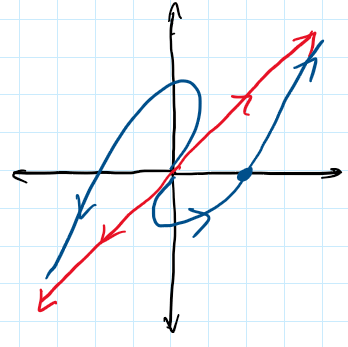
\includegraphics[height=1.5in]{Images/phaseportrait_5_n3_3_n1_sketch.png}}\hfill\hfill
%}

\begin{exercise}
    Solve the initial value problem
    \[ 
        {\vec{x}}' = 
        \begin{bmatrix} 
            -3 & 2 \\ 
            0 & -3 
        \end{bmatrix} 
        \vec{x} \qquad \vec{x}(0) = 
        \begin{bmatrix} 
            2 \\ 
            1 
        \end{bmatrix} 
    \] 
    and sketch the phase portrait for this system.\\
    $\vec{x}(t) = \left[\begin{smallmatrix} \answer{(2t+2)}e^{-3t} \\ \answer{(2t+1)}e^{-3t} \end{smallmatrix}\right]$
\end{exercise}
%\comboSol
%{%
%$\vec{x}(t) = \left[\begin{smallmatrix} (2t+2)e^{-3t} \\ (2t+1)e^{-3t} \end{smallmatrix}\right]$ \hfill\raisebox{-0.5\height}{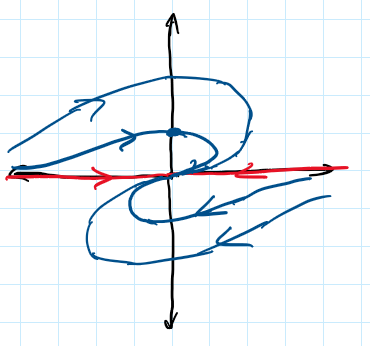
\includegraphics[height=1.5in]{Images/phaseportrait_n3_2_0_n3_sketch.png}}\hfill\hfill
%}


\begin{exercise}
    Solve the initial value problem
    \[ 
        {\vec{x}}' = 
        \begin{bmatrix} 
            -5 & -2 \\ 
            8 & 3 
        \end{bmatrix} 
        \vec{x} \qquad \vec{x}(0) = 
        \begin{bmatrix} 
            1 \\ 
            1 
        \end{bmatrix} 
    \] 
    and sketch the phase portrait for this system.\\
    $\vec{x}(t) = \left[\begin{smallmatrix} \answer{(-6t+1)e^{-t}} \\ \answer{(12t + 1)e^{-t}} \end{smallmatrix}\right]$
\end{exercise}
%\comboSol
%{%
%$\vec{x}(t) = \left[\begin{smallmatrix} (-6t+1)e^{-t} \\ (12t+1)e^{-t} \end{smallmatrix}\right]$ \hfill\raisebox{-0.5\height}{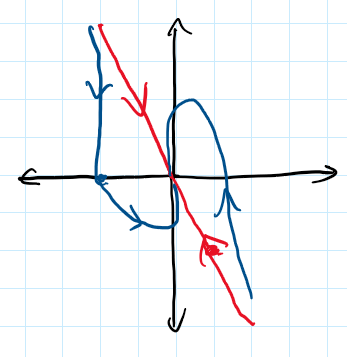
\includegraphics[height=1.5in]{Images/phaseportrait_n5_n2_8_3_sketch.png}}\hfill\hfill
%}

\begin{exercise}
    Solve the initial value problem
    \[ 
        {\vec{x}}' = 
        \begin{bmatrix} 
            -3 & -12 \\ 
            3 & 9 
        \end{bmatrix}
        \vec{x} \qquad \vec{x}(0) = 
        \begin{bmatrix} 
            3 \\ 
            2  
        \end{bmatrix} 
    \] 
    and sketch the phase portrait for this system.\\
    $\vec{x}(t) = \left[\begin{smallmatrix} \answer{(-42t + 3)e^{3t}} \\ \answer{(21t + 2)e^{3t}} \end{smallmatrix}\right]$
\end{exercise}
%\comboSol
%{%
%$\vec{x}(t) = \left[\begin{smallmatrix} (-42t+3)e^{3t} \\ (21t + 2)e^{3t} \end{smallmatrix}\right]$ \hfill\raisebox{-0.5\height}{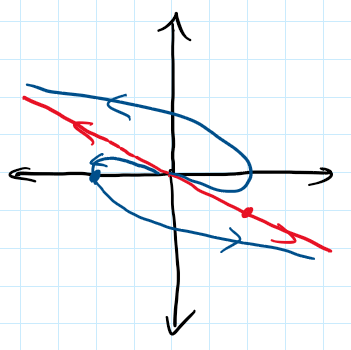
\includegraphics[height=1.5in]{Images/phaseportrait_n3_n12_3_9_sketch.png}}\hfill\hfill
%}

\begin{exercise}
    Assume $A$ is a $3\times 3$ matrix. The row-reduced echelon forms of $A-\lambda I$ are given for three different values of $\lambda$: $$A-3I \rightsquigarrow \begin{pmatrix} 1&0&0\\ 0&1&0\\ 0&0&1 \end{pmatrix} \qquad\qquad  A-5I \rightsquigarrow \begin{pmatrix} 1&4&0\\ 0&0&1\\ 0&0&0 \end{pmatrix}\qquad\qquad A-7I \rightsquigarrow \begin{pmatrix} 1&-1&1/2\\ 0&0&0\\ 0&0&0 \end{pmatrix}$$
    
    Find the general solution of the homogeneous system $\vec{x}'=A\vec{x}$.\\
    $\vec{x}(t) = C_1\left[\begin{smallmatrix} \answer{4} \\ -1 \\ \answer{0} \end{smallmatrix}\right]e^{5t} + C_2\left[\begin{smallmatrix} \answer{1} \\ 1 \\ \answer{0} \end{smallmatrix}\right]e^{7t} + C_2\left[\begin{smallmatrix} \answer{-\frac{1}{2}} \\ 0 \\ \answer{1} \end{smallmatrix}\right]e^{7t}$
\end{exercise}
%\comboSol
%{%
%$\vec{x}(t) = C_1\left[\begin{smallmatrix} 4 \\ -1 \\ 0 \end{smallmatrix}\right]e^{5t} + C_2\left[\begin{smallmatrix} 1 \\ 1 \\ 0 \end{smallmatrix}\right]e^{7t} + C_2\left[\begin{smallmatrix} -1/2 \\ 0 \\ 1 \end{smallmatrix}\right]e^{7t}$
%}

\begin{exercise}
    Consider the matrix
    $A=\displaystyle \begin{pmatrix} 
        7 & 5 & -6 \\
        0 & -3 & 2 \\
        0  & -4 & 1 
    \end{pmatrix}$
    \begin{itemize}
        \item Determine the characteristic polynomial of $A$ and give its eigenvalues.\\
            $\lambda = \answer{7}$, $\answer{-1}\pm \answer{2i}$
        \item How many (linearly independent) straight-line solutions does the system ${\vec{x}}'=A\vec{x}$ have? $\answer{1}$ %How do you know, without solving? 
    \end{itemize}
\end{exercise}
%\comboSol
%{%
%a)~$\lambda = 7,\ -1\pm 2i$ \quad b)~Only 1
%}

\begin{exercise}
    Let $A=\begin{bmatrix} 1&5&-18\\ 2&-1&-5 \\ 1&1&-6 \end{bmatrix}$. 
    \begin{itemize}
        \item Show directly that $\vec{v}_1=\begin{bmatrix} 1\\3\\1 \end{bmatrix}$ is an eigenvector of $A$.
        \item All eigenvalues of $A$ are the same. Find the general solution to ${\vec{x}}'=A\vec{x}$.\\
            $\vec{x}(t) = C_1\left[\begin{smallmatrix} \answer{1} \\ \answer{3} \\1 \end{smallmatrix}\right]e^{-2t} + C_2\left(\left[\begin{smallmatrix} \answer{1} \\ 3 \\ \answer{1} \end{smallmatrix}\right] te^{-2t} + \left[\begin{smallmatrix} \answer{2} \\ \answer{-1} \\ 0 \end{smallmatrix}\right]e^{-2t}\right) + C_3\left( \left[\begin{smallmatrix} \answer{1} \\ \answer{3} \\1 \end{smallmatrix}\right] \frac{t^2}{2}e^{-2t} + \left[\begin{smallmatrix} \answer{2} \\ -1 \\ \answer{0} \end{smallmatrix}\right]te^{-2t} + \left[\begin{smallmatrix} \answer{-1} \\ 1 \\ \answer{0} \end{smallmatrix}\right] e^{-2t}\right)$
    \end{itemize}
\end{exercise}
%\comboSol
%{%
%b)~$\vec{x}(t) = C_1\left[\begin{smallmatrix} 1 \\ 3 \\1 \end{smallmatrix}\right]e^{-2t} + C_2\left(\left[\begin{smallmatrix} 1 \\ 3 \\ 1 \end{smallmatrix}\right] te^{-2t} + \left[\begin{smallmatrix} 2 \\ -1 \\ 0 \end{smallmatrix}\right]e^{-2t}\right) + C_3\left( \left[\begin{smallmatrix} 1 \\ 3 \\1 \end{smallmatrix}\right] \frac{t^2}{2}e^{-2t} + \left[\begin{smallmatrix} 2 \\ -1 \\ 0 \end{smallmatrix}\right]te^{-2t} + \left[\begin{smallmatrix} -1 \\ 1 \\ 0 \end{smallmatrix}\right] e^{-2t}\right)$
%}


\begin{exercise}
    Let $A = 
    \left[ 
        \begin{smallmatrix}
            5 & -4 & 4 \\
            0 & 3 & 0 \\
            -2 & 4 & -1
        \end{smallmatrix} 
    \right]$.
    \begin{itemize}
        \item What are the eigenvalues? $\answer{3}$, $\answer{1}$, $\answer{1}$.
        \item How many defect(s) are there of the eigenvalue(s)? $\answer{0}$
        \item Find the general solution of ${\vec{x}}' = A \vec{x}$.\\
            $\vec{x}(t) = C_1\left[\begin{smallmatrix} \answer{1} \\ \answer{0} \\ -1 \end{smallmatrix}\right]e^t + C_2\left[\begin{smallmatrix} 2 \\ \answer{1} \\ \answer{0} \end{smallmatrix}\right]e^{3t} + C_3\left[\begin{smallmatrix} \answer{-2} \\ 0 \\ \answer{1} \end{smallmatrix}\right]e^{3t}$
    \end{itemize}
\end{exercise}
%\comboSol
%{%
%a)~3,1,1 \quad b)~No defects \quad c)~ $\vec{x}(t) = C_1\left[\begin{smallmatrix} 1 \\ 0 \\ -1 \end{smallmatrix}\right]e^t + C_2\left[\begin{smallmatrix} 2 \\ 1 \\ 0 \end{smallmatrix}\right]e^{3t} + C_3\left[\begin{smallmatrix} -2 \\ 0 \\ 1 \end{smallmatrix}\right]e^{3t}$
%}

\begin{exercise}%
    Let $A =
    \left[ 
        \begin{smallmatrix}
            1 & 1 & 1 \\
            1 & 1 & 1 \\
            1 & 1 & 1 
        \end{smallmatrix}
    \right]$.  
    \begin{itemize}
        \item What are the eigenvalues? $\answer{0}$, $\answer{0}$, $\answer{3}$
        \item How many defect(s) are there of the eigenvalue(s)? $\answer{0}$
        \item Find the general solution of $\vec{x}\,' = A\vec{x}$.\\
            $\vec{x} =
            C_1 \left[ \begin{smallmatrix}
                \answer{1} \\ \answer{1} \\ 1
            \end{smallmatrix}\right]
            e^{3t} + C_2
            \left[ \begin{smallmatrix}
                1 \\ \answer{0} \\ \answer{-1}
            \end{smallmatrix}\right] + C_3
            \left[ \begin{smallmatrix}
                0 \\ \answer{1} \\ \answer{-1}
            \end{smallmatrix}\right]$
    \end{itemize}
\end{exercise}
%\exsol{%
%a) $3,0,0$
%\quad
%b) No defects.
%\quad
%c)
%$\vec{x} =
%C_1
%\left[ \begin{smallmatrix}
%1 \\ 1 \\ 1
%\end{smallmatrix}\right]
%e^{3t}
%+
%C_2
%\left[ \begin{smallmatrix}
%1 \\ 0 \\ -1
%\end{smallmatrix}\right]
%+
%C_3
%\left[ \begin{smallmatrix}
%0 \\ 1 \\ -1
%\end{smallmatrix}\right]$
%}

\begin{exercise}
    Let
    $A = 
    \left[ 
        \begin{smallmatrix} 
            2 & 1 & 0 \\ 
            0 & 2 & 0 \\ 
            0 & 0 & 2 
        \end{smallmatrix} 
    \right]$.
    \begin{itemize}
        \item What are the eigenvalues? $\answer{2}$
        \item How many defect(s) are there of the eigenvalue(s)? $\answer{1}$
        \item Find the general solution of ${\vec{x}}' = A \vec{x}$ in two different ways and verify you get the same answer.\\
            $\vec{x}(t) = C_1 \left[\begin{smallmatrix} \answer{1} \\ \answer{0} \\ 0 \end{smallmatrix}\right]e^{2t} + C_2\left[\begin{smallmatrix} \answer{0} \\ 0 \\ \answer{1} \end{smallmatrix}\right]e^{2t} + C_3\left(\left[\begin{smallmatrix} \answer{1} \\ \answer{0} \\ 0 \end{smallmatrix}\right]te^{2t} + \left[\begin{smallmatrix} \answer{0} \\ 1 \\ \answer{0} \end{smallmatrix}\right]e^{2t}\right)$
    \end{itemize}
\end{exercise}
%\comboSol
%{%
%a)~2 \quad b)~Defect 1 \quad c)~$\vec{x}(t) = C_1 \left[\begin{smallmatrix} 1 \\ 0 \\ 0 \end{smallmatrix}\right]e^{2t} + C_2\left[\begin{smallmatrix} 0 \\ 0 \\ 1 \end{smallmatrix}\right]e^{2t} + C_3\left(\left[\begin{smallmatrix} 1 \\ 0 \\ 0 \end{smallmatrix}\right]te^{2t} + \left[\begin{smallmatrix} 0 \\ 1 \\ 0 \end{smallmatrix}\right]e^{2t}\right)$
%}

\begin{exercise}%
    Let $A =
    \left[ 
        \begin{smallmatrix}
            1 & 3 & 3 \\
            1 & 1 & 0 \\
            -1 & 1 & 2 \\
        \end{smallmatrix}
    \right]$.  
    \begin{itemize}
        \item What are the eigenvalues? $\answer{1}$, $\answer{1}$, $\answer{2}$
        \item How many defect(s) are there of the eigenvalue(s)? $\answer{2}$
        \item Find the general solution of $\vec{x}\,' = A\vec{x}$.\\
            $\vec{x} = C_1
            \left[ \begin{smallmatrix}
                \answer{0} \\ \answer{1} \\ -1
            \end{smallmatrix}\right]
            e^{t} + C_2
            \left(
                \left[ \begin{smallmatrix}
                    1 \\ \answer{0} \\ \answer{0}
                \end{smallmatrix}\right]
                + t 
                \left[ \begin{smallmatrix}
                    \answer{0} \\ 1 \\ \answer{-1}
                \end{smallmatrix}\right]
            \right)
            e^{t} + C_3
            \left[ \begin{smallmatrix}
                3 \\ \answer{3} \\ \answer{-2}
            \end{smallmatrix}\right]
            e^{2t}$
    \end{itemize}
\end{exercise}
%\exsol{%
%a) $1,1,2$
%\quad
%b) Eigenvalue 1 has a defect of 1
%\\
%c)
%$\vec{x} =
%C_1
%\left[ \begin{smallmatrix}
%0 \\ 1 \\ -1
%\end{smallmatrix}\right]
%e^{t}
%+
%C_2
%\left(
%\left[ \begin{smallmatrix}
%1 \\ 0 \\ 0
%\end{smallmatrix}\right]
%+
%t
%\left[ \begin{smallmatrix}
%0 \\ 1 \\ -1
%\end{smallmatrix}\right]
%\right)
%e^{t}
%+
%C_3
%\left[ \begin{smallmatrix}
%3 \\ 3 \\ -2
%\end{smallmatrix}\right]
%e^{2t}$
%}

\begin{exercise}
    Let $A = 
    \left[ 
        \begin{smallmatrix}
            0 & 1 & 2 \\
            -1 & -2 & -2 \\
            -4 & 4 & 7
        \end{smallmatrix} 
    \right]$.
    \begin{itemize}
        \item What are the eigenvalues? $\answer{1}$
        \item How many defect(s) are there of the eigenvalue(s)? $\answer{1}$
        \item Find the general solution of ${\vec{x}}' = A \vec{x}$.\\
            $\vec{x}(t) = C_1\left[\begin{smallmatrix} \answer{-2} \\ \answer{0} \\ 1 \end{smallmatrix}\right]e^{-t} + C_2\left[\begin{smallmatrix} 1 \\ \answer{-1} \\ \answer{2} \end{smallmatrix}\right]e^{3t} + C_3\left(\left[\begin{smallmatrix} 1 \\ \answer{-1} \\ \answer{2} \end{smallmatrix}\right]te^{3t} + \left[\begin{smallmatrix} \answer{0} \\ \answer{0} \\ \frac{1}{2} \end{smallmatrix}\right]e^{3t}\right)$
    \end{itemize}
\end{exercise}
%\comboSol
%{%
%a)~-1, 3\quad b)~3 has defect 1 \quad c)~$\vec{x}(t) = C_1\left[\begin{smallmatrix} -2 \\ 0 \\ 1 \end{smallmatrix}\right]e^{-t} + C_2\left[\begin{smallmatrix} 1 \\ -1 \\ 2 \end{smallmatrix}\right]e^{3t} + C_3\left(\left[\begin{smallmatrix} 1 \\ -1 \\ 2 \end{smallmatrix}\right]te^{3t} + \left[\begin{smallmatrix} 0 \\ 0 \\ 1/2 \end{smallmatrix}\right]e^{3t}\right)$
%}

\begin{exercise}%
    Let $A = \left[ 
        \begin{smallmatrix}
            2 & 0 & 0 \\
            -1 & -1 & 9 \\
            0 & -1 & 5
        \end{smallmatrix}
    \right]$.  
    \begin{itemize}
        \item What are the eigenvalues? $\answer{2}$, $\answer{2}$, $\answer{2}$
        \item How many defect(s) are there of the eigenvalue(s)? $\answer{3}$
        \item Find the general solution of $\vec{x}\,' = A\vec{x}$.\\
        $\vec{x} =
        C_1
        \left[ \begin{smallmatrix}
            \answer{0} \\ 3 \\ \answer{1}
        \end{smallmatrix}\right]
        e^{2t} + C_2
        \left(
            \left[ \begin{smallmatrix}
                0 \\ \answer{-1} \\ \answer{0}
            \end{smallmatrix}\right]
            + t
            \left[ \begin{smallmatrix}
                \answer{0} \\ 3 \\ \answer{1}
            \end{smallmatrix}\right]
        \right)
        e^{2t} + C_3
        \left(
            \left[ \begin{smallmatrix}
                \answer{1} \\ \answer{0} \\ 0
            \end{smallmatrix}\right]
            + t
            \left[ \begin{smallmatrix}
                0 \\ \answer{-1} \\ \answer{0}
            \end{smallmatrix}\right]
            + \frac{t^2}{2}
            \left[ \begin{smallmatrix}
                \answer{0} \\ 3 \\ \answer{1}
            \end{smallmatrix}\right]
        \right)
        e^{2t}$
    \end{itemize}
\end{exercise}
%\exsol{%
%a) $2,2,2$
%\quad
%b) Eigenvalue 2 has a defect of 2
%\\
%c)
%$\vec{x} =
%C_1
%\left[ \begin{smallmatrix}
%0 \\ 3 \\ 1
%\end{smallmatrix}\right]
%e^{2t}
%+
%C_2
%\left(
%\left[ \begin{smallmatrix}
%0 \\ -1 \\ 0
%\end{smallmatrix}\right]
%+
%t
%\left[ \begin{smallmatrix}
%0 \\ 3 \\ 1
%\end{smallmatrix}\right]
%\right)
%e^{2t}
%+
%C_3
%\left(
%\left[ \begin{smallmatrix}
%1 \\ 0 \\ 0
%\end{smallmatrix}\right]
%+
%t
%\left[ \begin{smallmatrix}
%0 \\ -1 \\ 0
%\end{smallmatrix}\right]
%+
%\frac{t^2}{2}
%\left[ \begin{smallmatrix}
%0 \\ 3 \\ 1
%\end{smallmatrix}\right]
%\right)
%e^{2t}$
%}

\begin{exercise}
    Let $A = 
    \left[ 
        \begin{smallmatrix}
            0 & 4 & -2 \\
            -1 & -4 & 1 \\
            0 & 0 & -2
        \end{smallmatrix} 
    \right]$.
    \begin{itemize}
        \item What are the eigenvalues? $\answer{2}$
        \item How many defect(s) are there of the eigenvalue(s)? $\answer{1}$
        \item Find the general solution of ${\vec{x}}' = A \vec{x}$.\\
            $\vec{x}(t) = C_1 \left[\begin{smallmatrix} \answer{1} \\ \answer{0} \\ 1 \end{smallmatrix}\right]e^{-2t} + C_2\left[\begin{smallmatrix} 0 \\ \answer{1} \\ \answer{2} \end{smallmatrix}\right]e^{-2t} + C_3\left( \left[\begin{smallmatrix} \answer{2} \\ -1 \\ \answer{0} \end{smallmatrix}\right]te^{-2t} + \left[\begin{smallmatrix} \answer{1} \\ \answer{0} \\ 0 \end{smallmatrix}\right]e^{-2t}\right)$
    \end{itemize}
\end{exercise}
%\comboSol
%{%
%a)~-2 \quad b)~Defect 1 \quad c)~$\vec{x}(t) = C_1 \left[\begin{smallmatrix} 1 \\ 0 \\ 1 \end{smallmatrix}\right]e^{-2t} + C_2\left[\begin{smallmatrix} 0 \\1 \\ 2 \end{smallmatrix}\right]e^{-2t} + C_3\left( \left[\begin{smallmatrix} 2 \\ -1 \\ 0 \end{smallmatrix}\right]te^{-2t} + \left[\begin{smallmatrix} 1 \\ 0 \\ 0 \end{smallmatrix}\right]e^{-2t}\right)$
%}

\begin{exercise}
    Let $A = 
    \left[ 
        \begin{smallmatrix}
            2 & 1 & -1 \\
            -1 & 0 & 2 \\
            -1 & -2 & 4
        \end{smallmatrix} 
    \right]$.
    \begin{itemize}
        \item What are the eigenvalues? $\answer{2}$
        \item How many defect(s) are there of the eigenvalue(s)? $\answer{1}$
        \item Find the general solution of ${\vec{x}}' = A \vec{x}$.\\
            $\vec{x}(t) = C_1 \left[\begin{smallmatrix} \answer{0} \\ \answer{1} \\ 1 \end{smallmatrix}\right]e^{2t} + C_2\left(\left[\begin{smallmatrix} 0 \\ \answer{1} \\ \answer{1} \end{smallmatrix}\right]te^{2t} + \left[\begin{smallmatrix} \answer{-1} \\ 0 \\ \answer{0} \end{smallmatrix}\right]e^{2t}\right) + C_3\left(\left[\begin{smallmatrix} \answer{0} \\1 \\ \answer{1} \end{smallmatrix}\right]\frac{t^2}{2}e^{2t} + \left[\begin{smallmatrix} \answer{-1} \\ \answer{0} \\ 0 \end{smallmatrix}\right]te^{2t} + \left[\begin{smallmatrix} -1 \\ \answer{-1} \\ \answer{0} \end{smallmatrix}\right]e^{2t}\right)$
    \end{itemize}
\end{exercise}
%\comboSol
%{%
%a)~2 \quad b)~ Defect of 2 \\ c)~ $\vec{x}(t) = C_1 \left[\begin{smallmatrix} 0 \\ 1 \\ 1 \end{smallmatrix}\right]e^{2t} + C_2\left(\left[\begin{smallmatrix} 0 \\1 \\ 1 \end{smallmatrix}\right]te^{2t} + \left[\begin{smallmatrix} -1 \\ 0 \\ 0 \end{smallmatrix}\right]e^{2t}\right) + C_3\left(\left[\begin{smallmatrix} 0 \\1 \\ 1 \end{smallmatrix}\right]\frac{t^2}{2}e^{2t} + \left[\begin{smallmatrix} -1 \\ 0 \\ 0 \end{smallmatrix}\right]te^{2t} + \left[\begin{smallmatrix} -1 \\-1 \\0 \end{smallmatrix}\right]e^{2t}\right)$
%}

\begin{exercise}
    Suppose that $A$ is a $2 \times 2$ matrix with a repeated eigenvalue $\lambda$. Suppose that there are two linearly independent eigenvectors.  Show that $A = \lambda I$.
\end{exercise}
%\comboSol
%{%
%Hint: This means everything is an eigenvector. Or, this can be set up as a system of equations.
%}

\begin{exercise}%
    Let $A =
    \left[ 
        \begin{smallmatrix}
            a & a \\
            b & c
        \end{smallmatrix}
    \right]$, 
    where $a$, $b$, and $c$ are unknowns. Suppose that $5$ is a doubled eigenvalue of defect 1, and suppose that
    $\left[ 
        \begin{smallmatrix}
            1 \\ 
            0
        \end{smallmatrix}
    \right]$ 
    is a corresponding eigenvector.  Find $A$ and show that there is only one such matrix $A$.\\
        $A = \left[ \begin{smallmatrix}
            \answer{5} & \answer{5} \\ \answer{0} & \answer{5}
        \end{smallmatrix}\right]$
\end{exercise}
%\exsol{%
%$A = \left[ \begin{smallmatrix}
%5 & 5 \\ 0 & 5
%\end{smallmatrix}\right]$
%}

\begin{exercise}%
    For each system, (i) classify the system according to type as one of sink/source/saddle/center/ spiral source/spiral sink; (ii) solve the systems; (iii) sketch the phase portrait. Both real and complex eigenvalues appear. %4.4, 4.5
    \begin{itemize}
        \item $\vec{x}'=\begin{pmatrix} 2&0 \\ 1&1 \end{pmatrix}\vec{x}$ %source
            \begin{multipleChoice}
                \choice{sink}
                \choice[correct]{source}
                \choice{saddle}
                \choice{center}
                \choice{spiral source}
                \choice{spiral sink}
                \choice{improper source}
            \end{multipleChoice}
            Solution: $C_1\left[\begin{smallmatrix} \answer{1} \\ \answer{1} \end{smallmatrix}\right]e^{2t} + C_2\left[\begin{smallmatrix} \answer{0} \\ 1 \end{smallmatrix}\right]e^t$  \\
            
        \item $\vec{x}'=\begin{pmatrix} -2& -2\\ 8& -2\end{pmatrix}\vec{x}$ %spiral sink
            \begin{multipleChoice}
                \choice{sink}
                \choice{source}
                \choice{saddle}
                \choice{center}
                \choice{spiral source}
                \choice[correct]{spiral sink}
                \choice{improper source}
            \end{multipleChoice}
            Solution:  $C_1e^{-2t}\left[\begin{smallmatrix} \answer{-\sin(4t)} \\ 2\cos(4t) \end{smallmatrix}\right] + C_2e^{-2t}\left[\begin{smallmatrix} \cos(4t) \\ \answer{2\sin(4t)} \end{smallmatrix}\right]$ \\
            
        \item $\vec{x}'=\begin{pmatrix} 3& 5\\ -5& -3  \end{pmatrix}\vec{x}$ %center
            \begin{multipleChoice}
                \choice{sink}
                \choice{source}
                \choice{saddle}
                \choice[correct]{center}
                \choice{spiral source}
                \choice{spiral sink}
                \choice{improper source}
            \end{multipleChoice}
            Solution:  $C_1\left[\begin{smallmatrix} 5\cos(4t) \\ \answer{-3\cos(4t)} + 4\sin(4t) \end{smallmatrix}\right] + C_2 \left[\begin{smallmatrix} 5\sin(4t)\\ 4\cos(4t) - \answer{3\sin(4t)} \end{smallmatrix}\right]$ \\
            
        \item $\vec{x}' = \begin{pmatrix} -1 & -3 \\ 3 & -7 \end{pmatrix}\vec{x}$ % Improper source
            \begin{multipleChoice}
                \choice{sink}
                \choice{source}
                \choice{saddle}
                \choice{center}
                \choice{spiral source}
                \choice{spiral sink}
                \choice[correct]{improper source}
            \end{multipleChoice}
            Solution: $C_1\left[\begin{smallmatrix} \answer{1} \\ 1 \end{smallmatrix}\right]e^{4t} + C_2\left(\left[\begin{smallmatrix} 1 \\ \answer{1}  \end{smallmatrix}\right]te^{4t} + \left[\begin{smallmatrix} \answer{\frac{1}{3}} \\ 0 \end{smallmatrix}\right]e^{4t}\right)$  \\
            
        \item $\vec{x}'=\begin{pmatrix} 3& 2\\ 0&-2 \end{pmatrix}\vec{x}$ %saddle
            \begin{multipleChoice}
                \choice{sink}
                \choice{source}
                \choice[correct]{saddle}
                \choice{center}
                \choice{spiral source}
                \choice{spiral sink}
                \choice{improper source}
            \end{multipleChoice}
            Solution: $C_1\left[\begin{smallmatrix} 1 \\ \answer{0} \end{smallmatrix}\right]e^{3t} + C_2\left[\begin{smallmatrix} \answer{2} \\ -5 \end{smallmatrix}\right]e^{-2t}$  \\
            
        \item $\vec{x}'=\begin{pmatrix} 2& \frac{1}{2} \\-1 & 1  \end{pmatrix}\vec{x}$ %spiral source
            \begin{multipleChoice}
                \choice{sink}
                \choice{source}
                \choice{saddle}
                \choice{center}
                \choice[correct]{spiral source}
                \choice{spiral sink}
                \choice{improper source}
            \end{multipleChoice}
            Solution: $C_1e^{\frac{3}{2}t}\left[\begin{smallmatrix} \answer{\cos(\frac{t}{2})} \\ \cos(\frac{t}{2}) - \sin(\frac{t}{2}) \end{smallmatrix}\right] + C_2e^{\frac{3}{2}t}\left[\begin{smallmatrix} \answer{\sin(\frac{t}{2})} \\ \sin\left(\frac{t}{2}\right) + \answer{\cos(\frac{t}{2})} \end{smallmatrix}\right]$  \\
            
        \item $\vec{x}'=\begin{pmatrix} 3& \frac{3}{2}\\ \frac{3}{2} & -1 \end{pmatrix}\vec{x}$ %saddle
            \begin{multipleChoice}
                \choice{sink}
                \choice{source}
                \choice[correct]{saddle}
                \choice{center}
                \choice{spiral source}
                \choice{spiral sink}
                \choice{improper source}
            \end{multipleChoice}
            Solution: $C_1\left[\begin{smallmatrix} 3 \\ \answer{1} \end{smallmatrix}\right]e^{\frac{7}{2}t} + C_2\left[\begin{smallmatrix} \answer{-1} \\ 3 \end{smallmatrix}\right]e^{-\frac{3}{3}t}$  \\
            
    \end{itemize}
\end{exercise}
%\exsol{%
%(a) Nodal Source,\ $C_1\left[\begin{smallmatrix} 1 \\ 1 \end{smallmatrix}\right]e^{2t} + C_2\left[\begin{smallmatrix} 0 \\ 1 \end{smallmatrix}\right]e^t$ \hfill\raisebox{-0.5\height}{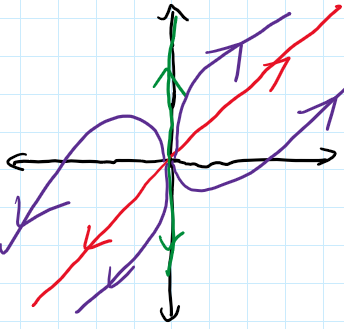
\includegraphics[height=1.5in]{Images/phaseportrait_2_0_1_1_sketch.png}}\hfill\hfill \\
%(b) Spiral Sink,\ $C_1e^{-2t}\left[\begin{smallmatrix} -\sin(4t) \\ 2\cos(4t) \end{smallmatrix}\right] + C_2e^{-2t}\left[\begin{smallmatrix} \cos(4t) \\ 2\sin(4t) \end{smallmatrix}\right]$ \hfill\raisebox{-0.5\height}{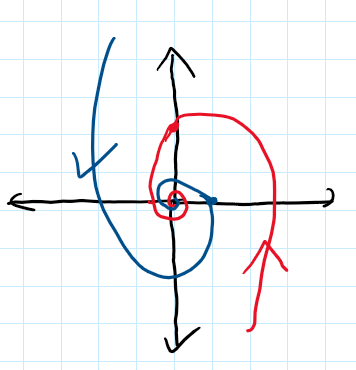
\includegraphics[height=1.5in]{Images/phaseportrait_n2_n2_8_n2_sketch.png}}\hfill\hfill\\
%(c) Center,\ $C_1\left[\begin{smallmatrix} 5\cos(4t) \\ -3\cos(4t) = 4\sin(4t) \end{smallmatrix}\right] + C_2 \left[\begin{smallmatrix} 5\sin(4t)\\ 4\cos(4t) - 3\sin(4t) \end{smallmatrix}\right]$ \hfill\raisebox{-0.5\height}{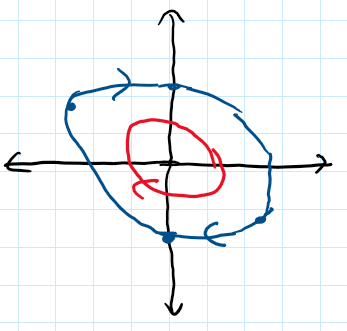
\includegraphics[height=1.5in]{Images/phaseportrait_3_5_n5_n3_sketch.png}}\hfill\hfill\\
%(d) Improper Nodal Source,\ $C_1\left[\begin{smallmatrix} 1 \\ 1 \end{smallmatrix}\right]e^{4t} + C_2\left(\left[\begin{smallmatrix} 1 \\ 1  \end{smallmatrix}\right]te^{4t} + \left[\begin{smallmatrix} 1/3 \\ 0 \end{smallmatrix}\right]e^{4t}\right)$ \hfill\raisebox{-0.5\height}{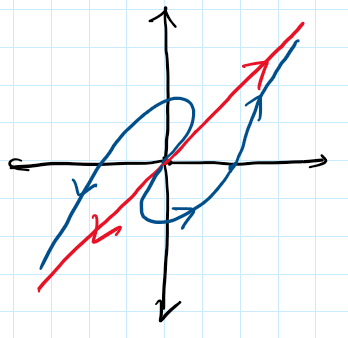
\includegraphics[height=1.5in]{Images/phaseportrait_n1_n3_3_n7_sketch.png}}\hfill\hfill\\
%(e) Saddle,\ $C_1\left[\begin{smallmatrix} 1 \\ 0 \end{smallmatrix}\right]e^{3t} + C_2\left[\begin{smallmatrix} 2 \\ -5 \end{smallmatrix}\right]e^{-2t}$ \hfill\raisebox{-0.5\height}{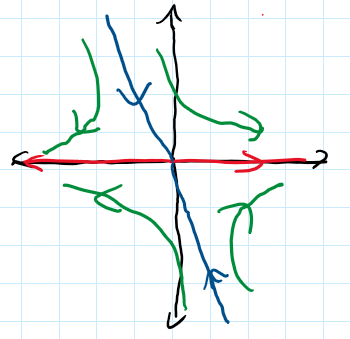
\includegraphics[height=1.5in]{Images/phaseportrait_3_2_0_n2_sketch.png}}\hfill\hfill\\
%(f) Spiral Source,\ $C_1e^{3t/2}\left[\begin{smallmatrix} \cos(t/2) \\ \cos(t/2) - \sin(t/2) \end{smallmatrix}\right] + C_2e^{3t/2}\left[\begin{smallmatrix} \sin(t/2) \\ \sin(t/2) + \cos(t/2) \end{smallmatrix}\right]$ \hfill\raisebox{-0.5\height}{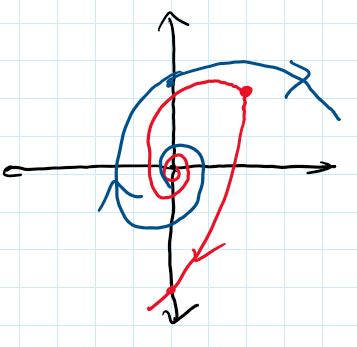
\includegraphics[height=1.5in]{Images/phaseportrait_2_h_n1_1_sketch.png}}\hfill\hfill\\
%(g) Saddle,\ $C_1\left[\begin{smallmatrix} 3 \\ 1 \end{smallmatrix}\right]e^{7t/2} + C_2\left[\begin{smallmatrix} -1 \\ 3 \end{smallmatrix}\right]e^{-3t/2}$ \hfill\raisebox{-0.5\height}{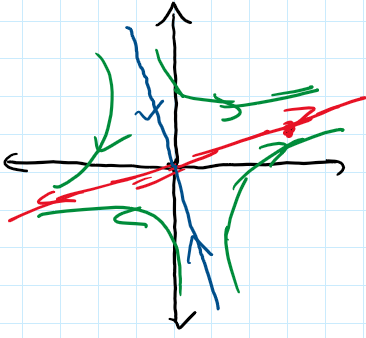
\includegraphics[height=1.5in]{Images/phaseportrait_3_3h_3h_n1_sketch.png}}\hfill\hfill
%}%

\begin{exercise}
    Consider the second order equation given by
    \begin{equation*}
        y'' + 2y' - 8y = 0.
    \end{equation*}
    \begin{itemize}
        \item Find the general solution of this problem using the methods of chapter \ref{ho:chapter}.
        \item Convert this equation into a first order linear system using the transformation $\vec{x} = \left[ \begin{smallmatrix} y \\ y' \end{smallmatrix} \right]$. \\
            ${\vec{x}}' = \left[\begin{smallmatrix} \answer{0} & 1 \\8 & \answer{-2} \end{smallmatrix}\right]\vec{x}$
        \item Find the eigenvalues and eigenvalues of the coefficient matrix and use that to find the general solution to the system.
        \item Extract the first component of the general solution and compare that to the solution from part (a). How do they relate?
        \item Look back through the work. How do the equation used to find the roots in (a) and the eigenvalues in (c) relate to each other?
    \end{itemize}
\end{exercise}
%\comboSol
%{%
%b)~${\vec{x}}' = \left[\begin{smallmatrix} 0 & 1 \\8 & -2 \end{smallmatrix}\right]\vec{x}$ \quad d)~It's the same!
%}

\begin{exercise}
    Consider the second order equation given by
    \begin{equation*}
        y'' + 4y' + 5y = 0.
    \end{equation*}
    \begin{itemize}
        \item Find the general solution of this problem using the methods of chapter \ref{ho:chapter}.
        \item Convert this equation into a first order linear system using the transformation $\vec{x} = \left[ \begin{smallmatrix} y \\ y' \end{smallmatrix} \right]$. \\
            ${\vec{x}}' = \left[\begin{smallmatrix} \answer{0} & 1 \\ \answer{-4} & \answer{-4} \end{smallmatrix}\right]\vec{x}$
        \item Find the eigenvalues and eigenvalues of the coefficient matrix and use that to find the general solution to the system.
        \item Extract the first component of the general solution and compare that to the solution from part (a). How do they relate?
        \item Look back through the work. How do the equation used to find the roots in (a) and the eigenvalues in (c) relate to each other?
    \end{itemize}
\end{exercise}
%\comboSol
%{%
%b)~${\vec{x}}' = \left[\begin{smallmatrix} 0 & 1 \\-4 & -4 \end{smallmatrix}\right]\vec{x}$ \quad d)~It's the same, up to potentially needing to rename the constants ($D_1 = 2C_1 + C_2$ and $D_2 = 2C_2 - C_1$)
%}

\begin{exercise}
    Consider the second order equation given by
    \begin{equation*}
        y'' - 4y' + 4y = 0.
    \end{equation*} for $b$ and $c$ two real numbers.
    \begin{itemize}
        \item Find the general solution of this problem using the methods of chapter \ref{ho:chapter}.
        \item Convert this equation into a first order linear system using the transformation $\vec{x} = \left[ \begin{smallmatrix} y \\ y' \end{smallmatrix} \right]$. \\
            ${\vec{x}}' = \left[\begin{smallmatrix} \answer{0} & 1 \\ \answer{-4} & 4 \end{smallmatrix}\right]\vec{x}$
        \item Find the eigenvalues and eigenvalues of the coefficient matrix and use that to find the general solution to the system.
        \item Extract the first component of the general solution and compare that to the solution from part (a). How do they relate?
        \item Look back through the work. How do the equation used to find the roots in (a) and the eigenvalues in (c) relate to each other?
    \end{itemize}
\end{exercise}
%\comboSol
%{%
%b)~${\vec{x}}' = \left[\begin{smallmatrix} 0 & 1 \\-4 & 4 \end{smallmatrix}\right]\vec{x}$ \quad d)~It's the same, up to potentially renaming the constants.
%}



\end{document}